\documentclass{article}

\usepackage[spanish, activeacute]{babel}

\usepackage{float}

\usepackage{graphicx}
\graphicspath{ {Imgs/} }

\usepackage{vmargin}

\setmargins{2.5cm}       % margen izquierdo
{1.0cm}                        % margen superior
{16.5cm}                      % anchura del texto
{23.42cm}                    % altura del texto
{10pt}                           % altura de los encabezados
{1cm}                           % espacio entre el texto y los encabezados
{0pt}                             % altura del pie de p'agina
{2cm}                           % espacio entre el texto y el pie de p'agina

\begin{document}
    \begin{center}
    	\huge \textbf{Escondite}
    \end{center}
    
    \hfill \break
    \large{ \textbf{Soluci'on}}

    \hfill \break
    Lo que nos pide el problema es encontrar el escondite mas al este. Para eso comenzaremos buscando
    de derecha a izquierda, as'i que lo primero es llegar al fondo. 

    Para empezar veamos como llegar a la segunda fila. Veamos el siguiente caso:

    \begin{figure}[h]
        \centering
        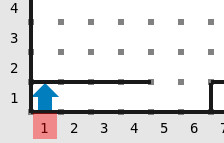
\includegraphics[scale=0.5]{primer_bloqueado}
    \end{figure}

    Como podemos tener el principio bloqueado, lo que h'aremos es orientarnos al este y avanzar hasta
    tener nuestra izquierda libre o hasta que no podamos avanzar m'as.

    Si nunca tuvimos la izquierda libre y llegamos a una pared, quiere decir que no podemos salir.

    \begin{figure}[h]
        \centering
        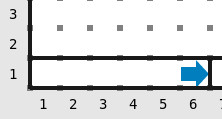
\includegraphics[scale=0.5]{imposible_salir}
    \end{figure}

    En ese caso la soluci'on es regresar a la casilla (1,1) y apagarse.

    \begin{figure}[h]
        \centering
        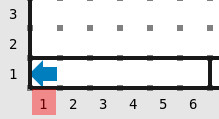
\includegraphics[scale=0.5]{regresando_a_1_1}
    \end{figure}

    Pero si en algun momento tenemos la izquierda libre, s'olo debemos orientarnos al norte y avanzar para salir
    a la fila 2.

    \begin{figure}[H]
        \centering
        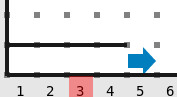
\includegraphics[scale = 0.5]{izquierda_libre}
    \end{figure}

    ahora solo hay que orientarse al este y avanzar hasta llegar a la pared. 

    \hfill \break
    \hfill \break
    \hfill \break
    \hfill \break
    \hfill \break
    \hfill \break
    \hfill \break

    Existen dos casos:

    \begin{enumerate}
    	\item La 'ultima casilla del parque est'a libre.
            \begin{figure}[H]
                \centering
                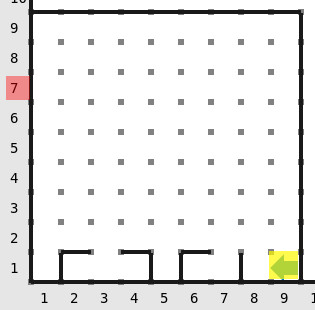
\includegraphics[scale=0.5]{ultima_libre}
            \end{figure}

            Este caso es sencillo porque lo 'unico que hay que hacer es orientarse al sur y avanzar.
    		
    	\item La 'ultima casilla del parque est'a bloqueada.
            \begin{figure}[H]
                \centering
                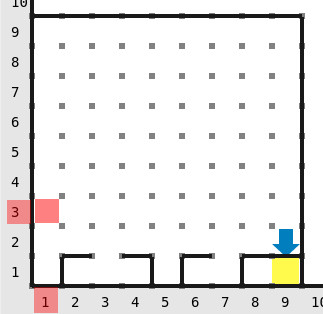
\includegraphics[scale=0.5]{ultima_bloqueada}
            \end{figure}

            Si esto pasa deberemos orientarnos al oeste y avanzar hasta que karel tenga su izquierda libre.

            \begin{figure}[H]
                \centering
                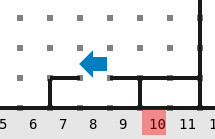
\includegraphics[scale=0.5]{ultima_bloqueada_izquierda_libre}
            \end{figure}

            ahora lo 'unico que hay que hacer es orientarse al sur y avanzar.
    \end{enumerate}

    Hasta ahora ya nos hemos posiciando correctamente, s'olo falta buscar el primer escondite avanzando de
    derecha a izquierda. Para eso avanzaremos siempre y cuando no tengamos una pared enfrente.

    \hfill \break
    \hfill \break

    Despu'es de avanzar si tenemos la derecha bloqueada (como en el siguiente ejemplo)
    entonces llegamos a nuestro destino y debemos apagarnos.

    \begin{figure}[H]
        \centering
        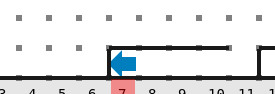
\includegraphics[scale=0.5]{escondite_bueno}
    \end{figure}

    Pero si no es as'i entonces tendremos que rodear la bardita. Para eso nos orientamos al norte, avanzamos,
    giramos a la izquierda y volvemos a avanzar.

    \begin{figure}[h]
        \centering
        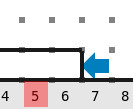
\includegraphics[scale=0.5]{primera_parte_saltar_barda}
    \end{figure}

    Ahora deberemos avanzar hasta tener la izquierda de karel libre. Para poder orientarnos al sur y avanzar para comenzar el proceso nuevamente.

    \begin{figure}[H]
        \centering
        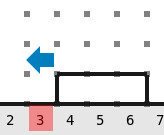
\includegraphics[scale=0.5]{segunda_parte_saltar_barda}
    \end{figure}

    Esto se repetir'a hasta que encontremos un escondite donde deberemos apagarnos.

    \begin{figure}[H]
        \centering
        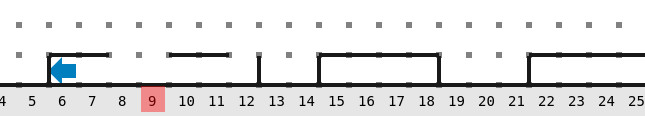
\includegraphics[scale=0.5]{escondite_bueno_2}
    \end{figure}
\end{document}